\documentclass[../../main.tex]{subfiles}

\begin{document}

\subsection{Overview}

This section contains a formal model describing the core parts of the system. The model was defined using \href{https://alloytools.org/}{Alloy}, an open source language and analyzer for software modelling. In particular, customers' line up, store access and store exit events are described.

The following additional assumptions have been added to the model for the sake of simplification, without significant loss of generality:
\begin{itemize}
  \item Time is quantized in time slots; the duration of the time slots is unspecified, thus it would be possible to shrink indefinitely the length of time slots to achieve a very fine level of precision;
  \item Customers leave the store within the time slot limits they requested during the line up request; this is a strong assumption that, however, can be mitigated by the system using the statistical data of the past visits of a customer to provide accurate estimations of the leaving time. In particular, during a line up request, the system could lookup the mean amount of time the customer spent in the store more than they were allowed in the past visits, and add it to the following line up requests.
\end{itemize}

The formal model shows that the system described in the present document:
\begin{itemize}
  \item is consistent with respect to the management of line up requests (i.e., it only accepts a line up request and emits the associated receipt if the requested store does not exceed the maximum number of customers allowed);
  \item is consistent with respect to the access to the store (i.e., it only allows a customer to enter the store if they have a valid line up receipt, they are using it for the first time to access the store and they are entering the store during the assigned time slot);
  \item is consistent with respect to the end of the visit to a store (i.e., it tracks the actual time slots the customer spent in the store);
  \item ensures that no more people than allowed are present inside each store.
\end{itemize}

\subsection{Alloy model}

\subsubsection{Source code}

// TODO: ATTACH CODE

\subsubsection{Predicates execution and assertions checks}

\begin{figure}[H]
  \centering
  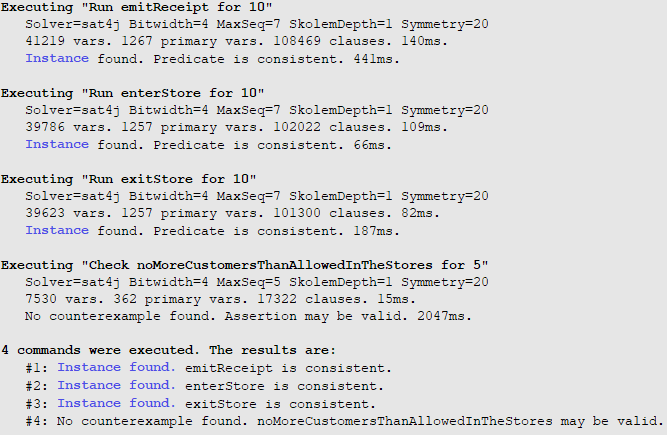
\includegraphics[width=\textwidth]{alloy_exec.png}
  \caption{Results of the execution of the Alloy predicates and assertions checks}
\end{figure}

\subsubsection{Resulting worlds}

\begin{figure}[H]
  \centering
  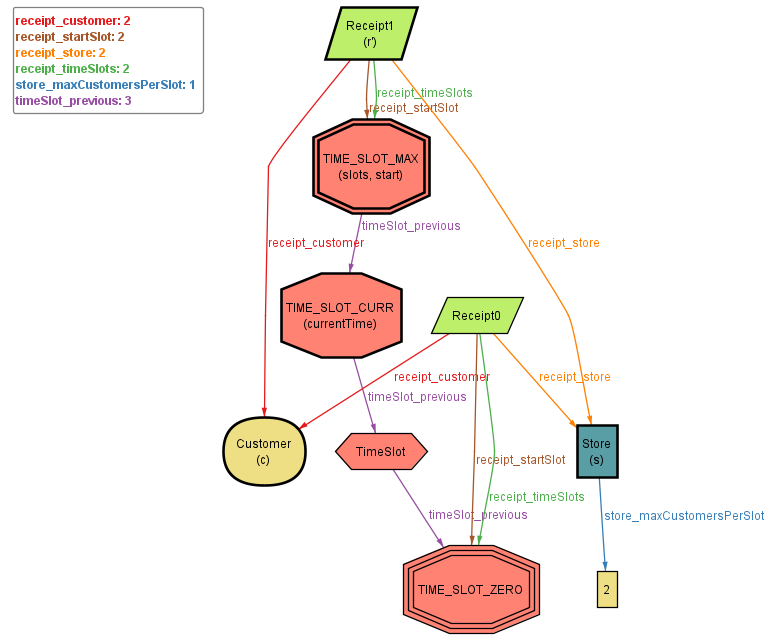
\includegraphics[width=\textwidth]{alloy_emitreceipt.png}
  \caption{One of the worlds generated by the emitReceipt predicate}
\end{figure}

\begin{figure}[H]
  \centering
  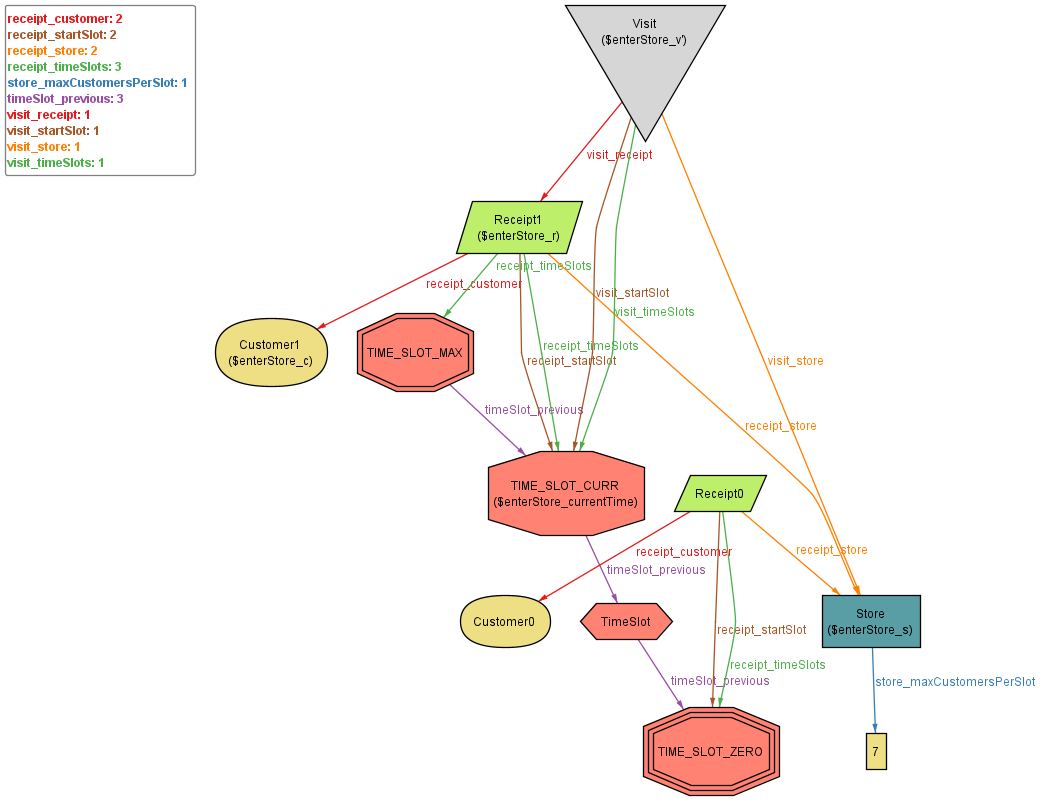
\includegraphics[width=\textwidth]{alloy_enterstore.png}
  \caption{One of the worlds generated by the enterStore predicate}
\end{figure}

\begin{figure}[H]
  \centering
  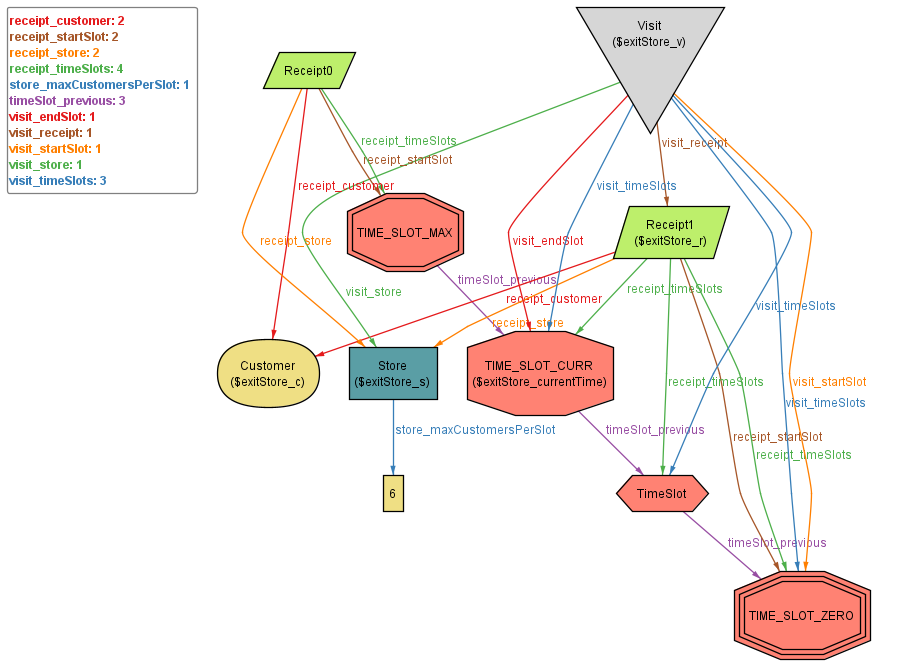
\includegraphics[width=\textwidth]{alloy_exitstore.png}
  \caption{One of the worlds generated by the exitStore predicate}
\end{figure}


\end{document}
